\documentclass{article}

\usepackage[T2A]{fontenc} % Кодировка шрифта
\usepackage[utf8]{inputenc} % Кодировка ввода
\usepackage[english,russian]{babel} % Языковые настройки
\usepackage{graphicx} % Для вставки изображений
\usepackage{amsmath} % Для использования математических формул
\usepackage{amssymb}
\usepackage{cancel}
\usepackage{amsfonts} % Для использования математических символов и шрифтов
\usepackage{titlesec} % Для настройки заголовков разделов
\usepackage{titling} % Для настройки титульной страницы
\usepackage{geometry} % Для настройки размеров страницы
\usepackage{pgfplots}
\pgfplotsset{compat=1.9}

% Настройка заголовков разделов
\titleformat{\section}
{\normalfont\Large\bfseries}{\arabic{section}}{1em}{}
\titleformat{\subsection}
{\normalfont\large\bfseries}{}{1em}{}

% Настройка титульной страницы
\setlength{\droptitle}{-3em} % Отступ заголовка
\title{\vspace{-1cm}ИДЗ №1}
\author{Вершинин Данил Алексеевич}
\date{\today}

% Настройка размеров страницы
\geometry{a4paper, margin=2cm}

\begin{document}
	
	% Автоматическая генерация оглавления (см. далее)
	\maketitle
	%\tableofcontents
	%\chapter{Задачи}
	\section{Найти все значения корня: $\sqrt[3]{8i}$}
	\subsection{Решение:}
	\[w= 8i\]
	Найду модуль и аргумент:
	\[\rho = |8i| = \sqrt{64} = 8 \\ \]
	\[\phi = \arctg\left(\frac{8}{0}\right) = \arctg(+\infty) = \frac{\pi}{2}\]
	\[2 = 8(\cos\left(\frac{\pi}{2}\right) + i \sin\left(\frac{\pi}{2}\right))\]
	\[z_k = 2 \left(\cos\left(\frac{\pi }{2\cdot 3} + \frac{2\pi k}{3}\right) + i \sin\left(\frac{\pi }{2\cdot 3} + \frac{2\pi k}{3}\right)\right) = 2 \left(\cos\left(\frac{\pi }{6} + \frac{2\pi k}{3}\right) + i \sin\left(\frac{\pi }{6} + \frac{2\pi k}{3}\right)\right)\]
	\[z_0 = 2 \left(\cos\left(\frac{\pi}{6}\right) + i \sin\left(\frac{\pi}{6}\right)\right) = \sqrt{3} + i\]
	\[z_1 = 2 \left(\cos\left(\frac{\pi}{6} + \frac{2\pi}{3}\right) + i \sin\left(\frac{\pi}{6} + \frac{2\pi}{3}\right)\right) = 2 \left(\cos\left(\frac{5\pi}{6}\right) + i \sin\left(\frac{5\pi}{6}\right)\right) = - \sqrt{3} + i\]
	\[z_2 = 2 \left(\cos\left(\frac{\pi}{6} + \frac{4\pi}{3}\right) + i \sin\left(\frac{\pi}{6} + \frac{4\pi}{3}\right)\right) = 2 \left(\cos\left(\frac{3\pi}{2}\right) + i \sin\left(\frac{3\pi}{2}\right)\right) = -2i\]
	\subsection{Ответ:}
	\[z_0 = \sqrt{3} + i\]
	\[z_1 = - \sqrt{3} + i\]
	\[z_3 = -2i\]
	
	\section{Представить в алгебраической форме: $\sh(2-\pi i)$}
	\subsection{Решение:}
	\[\sh(2-\pi) = \sh(2)\ch(\pi i) - \ch(2)\sh(\pi i) = -\sh(2)\]
	\[\ch(\pi i) = \cos(\pi) = -1\]
	\[\sh(i\pi) = i \sin(\pi) = 0\]
	\subsection{Ответ:}
	\[-\sh(2)\]
	
	\section{Представить в алгебраической форме: $\text{arcth}(1+ \sqrt{3}i)$}
	\subsection{Решение:}
	\[\text{arcth}(1+ \sqrt{3}i)\]
	\[\text{arcth}(z) = w \Rightarrow \cth(w) = z\]
	\[\frac{e^w + e^{-w}}{e^w - e^{-w}} = z\]
	\[\frac{e^w + 1/e^w}{e^w - 1/e^w} = \frac{e^{2w}+1}{e^{2w}-1} = z \Rightarrow e^{2w} + 1 = z \left(e^{2w} -1\right)\]
	\[e^{2w}(1-z) +z +1 = 0\]
	\[e^{2w}(1-z) + (z+1) = 0 \Rightarrow e^{2w} = \frac{z+1}{z-1}\]
	\[2w = \text{Ln}\left(\frac{z+1}{z-1}\right) = \ln \left|\frac{z+1}{z-1}\right| + i\text{Arg}\left(\frac{z+1}{z-1}\right) \]
	\[w=  \frac{1}{2} \left(\ln \left|\frac{z+1}{z-1}\right| + i\left(\text{arg}\left(\frac{z+1}{z-1}\right) +2\pi n\right)\right), \ n \in \mathbb{Z}\]
	\[\frac{z+1}{z-1} = \frac{2 + \sqrt{3}i}{\sqrt{3}i}\cdot \frac{-\sqrt{3}i}{-\sqrt{3}i} = \frac{3 - 2\sqrt{3}i}{3} = 1 - \frac{2\sqrt{3}i}{3}\]
	\[\left|\frac{z+1}{z-1} \right| = \left|1 - \frac{2\sqrt{3}i}{3}\right| = \sqrt{1 + \frac{4}{3}} = \sqrt{\frac{7}{3}}\]
	\[\text{arg}\left(1 -\frac{2\sqrt{3}i}{3}\right) = \arctg\left(-\frac{2}{\sqrt{3}}\right) = -\arctg\left(\frac{2}{\sqrt{3}}\right)\]
	\[w = \frac{1}{2} \left(\ln\sqrt{\frac{7}{3}} + i \left(-\arctg\left(\frac{2}{\sqrt{3}}\right) + 2\pi n\right)\right), \ n \in \mathbb{Z}\]
	\subsection{Ответ:}
	\[\frac{1}{2} \left(\ln\sqrt{\frac{7}{3}} + i \left(-\arctg\left(\frac{2}{\sqrt{3}}\right) + 2\pi n\right)\right), \ n \in \mathbb{Z}\]
	
	\section{Представить в алгебраической форме: $(-3i)^i$}
	\subsection{Решение:}
	\[(-3i)^i = e^{i\text{Ln}(-3i)}\]
	\[\text{Ln}(-3i) = \ln |-3i| + i\text{Arg}(-3i) = \ln(3) + i\left(-\frac{\pi}{2} + 2\pi k\right), k \in \mathbb{Z}\]
	\[e^{i\text{Ln}(-3i)} = e ^ {\left(\frac{\pi}{2} + 2\pi k\right) + i\ln(3)} = e ^ {\left(\frac{\pi}{2} + 2\pi k\right)}\left(\cos\left(\ln(3)\right) + i\sin\left(\ln(3)\right)\right), k \in \mathbb{Z}\]
	\subsection{Ответ:}
	\[e ^ {\left(\frac{\pi}{2} + 2\pi k\right)}\left(\cos\left(\ln(3)\right) + i\sin\left(\ln(3)\right)\right), k \in \mathbb{Z}\]
	
	\section{Представить в алгебраической форме: $\text{Ln}(2+2\sqrt{3}i)$}
	\subsection{Решение:}
	\[\text{Ln}(2+2\sqrt{3}i) = \ln|2 + 2\sqrt{3}i| + i\text{Arg}(2+2\sqrt{3}i) = \ln 4 + i\left(\frac{\pi}{3} + 2\pi k\right), k \in \mathbb{Z}\]
	\subsection{Ответ:}
	\[\ln 4 + i\left(\frac{\pi}{3} + 2\pi k\right), k \in \mathbb{Z}\]
	
	\section{Вычертить область, заданную неравествами: $\\D = \{z : |z - 1 + i| \ge 1, Re(z) < 1, Im(z) \le 1 \}$}
	\subsection{Ответ:}
	Пунктир
	\begin{figure}[h]
		\centering
		\begin{tikzpicture}
			
			\filldraw[draw=cyan, line width=1pt, fill=cyan!20] (-3, 1) -- (1,1) -- (1, 0) arc (90:270:1)--(1,-3)--(-3,-3)--(-3,0);
			\draw[blue!40] (1,-1) circle (1); % заливка круга с центром в (1,1) и радиусом 1
			\draw[thick, ->] (-3,0) -- (3,0) node[below] {$\Re(z)$};
			\draw[thick, ->] (0,-3) -- (0,2) node[left] {$\Im(z)$};
			\draw[thick] (1,-1)--(2, -1) node[midway,below]{1} ;
			\draw (-3, 1) -- (3,1);
			\filldraw (1,0) circle (2pt) node[above, right]{$1$};
			\filldraw (0,1) circle (2pt) node[above, right]{$i$};
			\draw[dashed] (1,2) -- (1,0); % линия Im(z) = 1
			\draw[dashed] (1,-2) -- (1, -3);
			
		\end{tikzpicture}
		\caption{Нужная нам область выделена голубым}
		
	\end{figure}
	
	
	
	
	\section{Определить вид пути и в случае, когда он проходит через точку $\infty$, исследовать его поведение в этой точке: $z = \frac{4}{\ch(4t)} + i2\th(4t)$}
	\subsection{Решение:}
	\[z = \frac{4}{\ch(4t)} + i2\th(4t)\]
	\[\begin{cases}
		x = \frac{4}{\ch(4t)} \\
		y = 2 \th(4t)
	\end{cases}\]
	\[x= \frac{4}{\ch (4t)} \Rightarrow \frac{x}{4} = \frac{1}{\ch (4t)} \Rightarrow \frac{x^2}{16} = \frac{1}{\ch^2 (4t)}\]
	\[y = 2 \th(4t) \Rightarrow \frac{y}{2} = \frac{\sh(4t)}{\ch(4t)} \Rightarrow\frac{y^2}{4} = \frac{\sh^2(4t)}{\ch^2(4t)} + 1 -1 \Rightarrow\frac{y^2}{4} = -\frac{1}{\ch(4t)}+1\]
	\[-\frac{y^2}{4} + 1 = \frac{1}{\ch^2(4t)}\]
	\[\frac{x^2}{16} = -\frac{y^2}{4} + 1 \Rightarrow \frac{x^2}{16} + \frac{y^2}{4} = 1\]
	\[t =0 : x \rightarrow 4, y \rightarrow 0\]
	\[t \rightarrow +\infty : x \rightarrow 0, y \rightarrow 2\]
	\[t \rightarrow -\infty : x \rightarrow 0, y \rightarrow -2\]
	
	
	\begin{figure}[h]
		\centering
		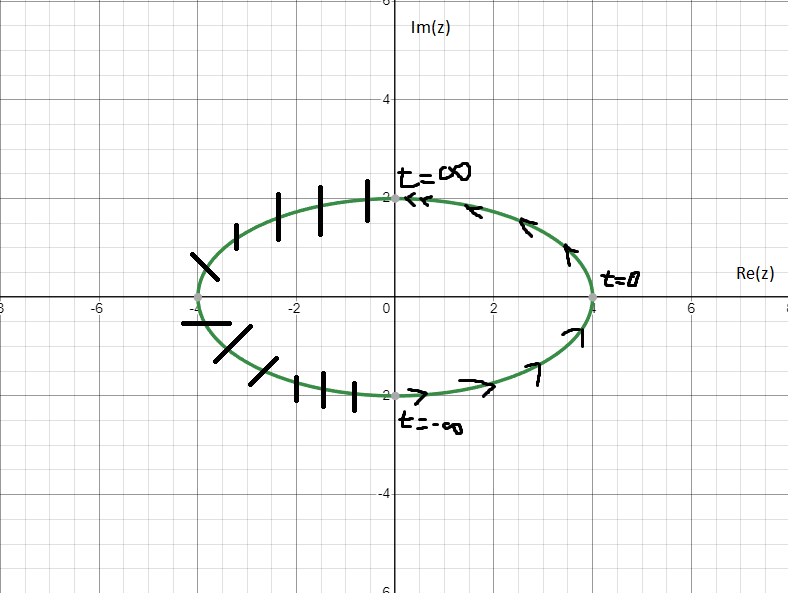
\includegraphics[width= 0.9\textwidth]	{7.png}
		\caption{z - эллипс. Левая часть не нужна, т.к. x не может принимать отрицательные значения}
		\label{fig:your_label}
	\end{figure}
	
	
	
	\section{Восстановить голоморфную в окрестности точки $z_0$ функцию $f(z)$ по известной действительной части $u(x,y)$ или мнимой $v(x,y)$ и начальному значению $f(z_0)$: $u = x^2 - y^2 + x, \ f(0) = 0$}
	\subsection{Решение:}
	\[u = x^2 - y^2 + x\]
	\[\frac{\delta u}{\delta x} = 2x+1\]
	\[\frac{\delta u}{\delta y} = -2y\]
	\[\begin{cases}
		\frac{\delta^2 u}{\delta x ^2} = 2\\
		\frac{\delta ^ 2 г}{\delta y^2} = -2
	\end{cases} \Rightarrow 2 -2 = 0 \text{- следовательно, условие Лапласа выполнено}\]
	Из условий Коши-Римана получаем систему дифференцальных уравнений, которая легко решается. Интегрируем второе уравнение по x:
	\[\begin{cases}
		\frac{\delta u }{\delta x} = \frac{\delta v}{\delta y} \\
		\frac{\delta u} {\delta y} = - \frac{\delta v}{\delta x}
	\end{cases} \Rightarrow
	\begin{cases}
		\frac{\delta v}{\delta y} = 2x+1 \\
		\frac{\delta v}{\delta x} = 2y
	\end{cases}\]
	\[v = 2yx + \phi (y) \ \Rightarrow \frac{\delta v}{\delta y} =2x + \phi'(y) \Rightarrow \phi' (y) = 1 \Rightarrow \phi(y) = y+C\]
	\[f(x,y) = u(x,y) + iv(x,y) = x^2 - y^2 +x + i (2xy + y + C)  = x + iy + x^2 - y^2 + 2ixy + iC =(*)\]
	\[z = x + iy \Rightarrow z ^2 = x^2 - y^2 +2ixy\]
	\[(*) = z + z^2 + iC\]
	\[f(0) = 0 \Rightarrow C = 0\]
	\[f(z) = z^2 + z\]
	\subsection{Ответ:}
	\[f(z) = z^2 + z\]
	
	\section{Вычислить интеграл от функции комплексной переменной по данному пути: $\int_{AB} z \Im(z^2) dz; \ AB - \text{отрезок прямой } z_A = 0, \ z_B = 1 + i$}
	\subsection{Решение:}
	\[z= x +iy \Rightarrow z ^2 = x^2 - y^2 + 2ixy \Rightarrow \Im(z^2) = 2xy\]
	\[z\Im (z^2) = (x+iy)(2xy) = 2x^2y + 2ixy^2\]
	\[Z_AZ_B: \begin{cases}
		x =t \\ y = t
	\end{cases}; 0 \le t \le 1; \ z(t) = t + it \Rightarrow z'(t) = 1 + i\]
	
	\[\int_{AB} z \Im(z^2) dz = \int\limits_{0}^1 (2x^2(t)y(t) + 2ix(t)y^2(t)) (1+i) dt = \int\limits_{0}^1 (2t^3 + 2it^3) (1+i) dt = \int\limits_{0}^1 2t^3(i+1)^2dt = \]
	\[ =2(1+i)^2\int\limits_{0}^1 t^3dt = \cancel{2}(1+i)^2\cdot\frac{1}{\cancel{4}_2} = \frac{1}{2}(\cancel{1} + 2i -\cancel{1}) = \frac{2i}{2} = i\]
	\subsection{Ответ:}
	$i$
	
	\section{Найти радиус сходимости степенного ряда: $\sum\limits_{n=1}^{\infty}(\cos^2(n))\cdot z^n$}
	\subsection{Решение:}
	\[\sum\limits_{n=1}^{\infty}(\cos^2(n))\cdot z^n\]
	\[\text{Радиус сходимости: }R = \frac{1}{\rho}, \text{ где } \rho = \overline{\underset{n\rightarrow\infty}{\lim}}\sqrt[n]{C_n}\]
	\[C_n = \cos^2n, \text{ очевидно, что }\cos^2n \le 1 \Rightarrow \overline{\underset{n\rightarrow\infty}{\lim}}\sqrt[n]{C_n} \le 1\]
	\[|C_n| \ \cancel{\rightarrow} \ 0 \Rightarrow \cos^2n \ \cancel{\rightarrow} \ 0 \eqno(*)\]
	\[\exists n_k \cos^2 n_k \underset{n_k \rightarrow \infty}{\rightarrow} \alpha \ne 0 \Rightarrow \overline{\underset{n_k \rightarrow\infty}{\lim}} \sqrt[n_k]{\cos^2 n_k} \ge \overline{\underset{n_k \rightarrow\infty}{\lim}} \sqrt[n_k]{\alpha}\]
	\[\overline{\underset{n_k\rightarrow\infty}{\lim}} \sqrt[n_k]{\alpha} \le \overline{\underset{n_k\rightarrow\infty}{\lim}} \sqrt[n_k]{\cos^2 n_k} \le 1 \Rightarrow\overline{\underset{n\rightarrow\infty}{\lim}}\sqrt[n]{\cos^2n} = 1\]
	\[(*): \text{ предположим противное: } \cos^2 n \underset{n \rightarrow \infty}{\rightarrow} 0 \Rightarrow \cos^2 (2n) \underset{n \rightarrow \infty}{\rightarrow} 0\]
	\[(\cos^2n -\sin^2n) \underset{n \rightarrow \infty}{\rightarrow} 0 \Rightarrow\begin{cases}
		\cos^2n \underset{n \rightarrow \infty}{\rightarrow} 0 \\
		\sin^2n \underset{n \rightarrow \infty}{\rightarrow} 0
	\end{cases}, \text{ но при этом } \cos^2 + \sin^2 = 1 \text{ - не выполнсяется.}\]\[\text{ Следовательно, получилм противоречие. } \Rightarrow \cos^2n \cancel{\rightarrow} 0, \text{ что и требовалось доказать.}\]
	Тогда получается, что $R = 1 / \rho = 1/ \ \overline{\underset{n\rightarrow\infty}{\lim}}\sqrt[n]{\cos^2n}  =1/1  = 1$
	\subsection{Ответ:}
	$R = 1$
	\section{Найти все лорановское разложение данной функции в 0 и в $\infty$: $f(z) = \frac{5z+100}{50z - 5z^2 -  z^3}$ (пример поправил, т.к. в ином случае корни не рациональные)}
	\subsection{Решение:}
	\[50z-5z^2-z^3 = 0 \Rightarrow z(50-5z-z^2)=0\]
	\[z_1=0,\ 50-5z-z^2 = 0\]
	\[z_{2,3} = \frac{5 \pm \sqrt{25+200}}{-2} =\begin{cases}
		-10,\\ 5
	\end{cases}\]
	\[\frac{5z+100}{50z-5z^2-z^3} =-\left( \frac{a}{z} + \frac{b}{z-5} + \frac{c}{z+10}\right) = (*)\]
	\[50a - 5az -az^2 - bz^2 - 10bz - cz^2 + 5cz=5z+100\]
	$z^2: \ a+b+c=0\Rightarrow b+c = -2\Rightarrow c =-1/3$\newline
	$z: \ -5a-10b + 5c = 5 \Rightarrow -2b + c = 3 \Rightarrow 3b=-5 \Rightarrow b = -5/3 $\newline
	$1: 50a =100 \Rightarrow a = 2$\newline
	\[(*) = \frac{2}{z} - \frac{5}{3(z-5)} - \frac{1}{3(z+10)}\]
	Первое слагаемое уже является разложением в ряд Лорана. Осталось найти разложение второго и третьего.\newline
	Для начала найдём разложение в окрестности нуля.\newline
	Заметим, что функция $\frac{5}{3(z-5)}$ - голоморфна при $|z| < 5$, следовательно, её ряд Лорана совпадает с рядом Тейлора (с кругом сходимости $|z| < 5$):
	\[\frac{5}{3(z-5)} = \frac{5}{15} \cdot \frac{-1}{(1-\frac{z}{5})}=\frac{-1}{3}\sum\limits_{n=0}^\infty \left(\frac{z}{5}\right)^n = \sum\limits_{n=0}^\infty \left(\frac{-1}{3}\cdot\frac{1}{5^n}z^n\right) \eqno(1)\]
	Аналогично расскладывается и третье слагаемое. Также отметим, что функция $\frac{1}{3(z+10)}$- голоморфна при $|z| < 10$. Отсюда получаем, что её ряд Лорена совпадает с рядом Тейлора (с кругом сходимости $|z| < 10$):
	\[\frac{1}{3(z+10)} = \frac{1}{30}\cdot\frac{1}{(1+\frac{z}{10})} = \frac{1}{30}\sum\limits_{n=0}^{\infty}(-1)^n\left(\frac{z}{10}\right)^n = \sum\limits_{n=0}^{\infty}\frac{1}{3}\frac{(-1)^n}{10^{n+1}}z^n\eqno(2)\]
	Формулы (1) и (2) справедливы при $|z| < 5$
	\[\frac{5z+100}{50z - 5z^2 -  z^3} = \frac{2}{z} + \sum\limits_{n=0}^\infty \left(\frac{1}{3}\cdot\frac{1}{5^n}z^n\right) - \sum\limits_{n=0}^{\infty}\frac{1}{3}\frac{(-1)^n}{10^{n+1}}z^n = \frac{2}{z} + \sum\limits_{n=0}^\infty \frac{1}{3}\left(\frac{1}{5^n} + \frac{(-1)^{n+1}}{10^{n+1}}\right)z^n\]
	Это выполняется в кольце $0 < z < 5$, где $C_n = \begin{cases}
		0, & n \le -2\\
		2, & n = -1\\
		\frac{1}{5^n} + \frac{(-1)^{n+1}}{10^{n+1}}, & n \ge 0 
	\end{cases}$ \newline
	Разложим теперь $\frac{5}{3(z-5)}$ в окрестности $\infty$. Очевидно, что эта функция голоморфна на $|z| > 5$. Поэтому преобразуем её так:
	\[\frac{5}{3(z-5)} = \frac{5}{3z} \cdot \frac{1}{(1-\frac{5}{z})}\]
	Заметим, что при $|z| > 5$ имеем $\left|\frac{5}{z}\right| < 1$ и поэтому получим:
	\[\frac{1}{1 - \frac{5}{z}} = \sum\limits_{n=0}^\infty \left(\frac{5}{z}\right)^n\]
	Окончательно получим:
	\[\frac{5}{3z} \cdot \frac{1}{1 - \frac{5}{z}} = \frac{5}{3z} \cdot \sum\limits_{n=0}^\infty \left(\frac{5}{z}\right)^n = \sum\limits_{n=0}^\infty \frac{5^{n+1}}{3z^{n+1}} =(\text{замена индекса (штрих стерли): } n+1 = -n') = \sum\limits_{n=-\infty}^{-1}\frac{z^n}{3\cdot 5^n}\eqno(3)\]
	Аналогично и при $|z| > 10$ разложение для $\frac{1}{3(z+10)}$(четвертое равенство - замена индекса $n+1=-n'$, штрих стерли):
	\[\frac{1}{3(z+10)} = \frac{1}{3z}\cdot\frac{1}{1+\frac{10}{z}} = \frac{1}{3z} \sum\limits_{n=0}^{\infty}(-1)^n \left(\frac{10}{z}\right)^n = \sum\limits_{n=0}^\infty \frac{(-1)^n 10^n}{3z^{n+1}} = \sum\limits_{n=-\infty}^{-1} \frac{z^n}{3(-1)^{n-1} 10^{n-1}}\eqno(4)\]
	Формулы (3) и (4) справедливы для $|z| > 10$ поэтому :
	\[\frac{5z+100}{50z - 5z^2 -  z^3} = \frac{2}{z} - \frac{5}{3(z-5)} - \frac{1}{3(z+10)} = \frac{2}{z} - \sum\limits_{n=-\infty}^{-1}\left(\frac{1}{3\cdot5^n} + \frac{1}{3(-1)^{n-1} 10^{n-1}}\right)z^n =\]
	\[=(\text{Вычислим сумму для }n =-1) =\frac{-33}{z} - \sum\limits_{n=-\infty}^{-2}\left(\frac{1}{3\cdot5^n} + \frac{1}{3(-1)^{n-1} 10^{n-1}}\right)z^n\]
	\subsection{Ответ:}
	В точке 0:\newline
	$\frac{2}{z} + \sum\limits_{n=0}^\infty \frac{1}{3}\left(\frac{1}{5^n} + \frac{(-1)^{n+1}}{10^{n+1}}\right)z^n$\newline\newline
	В точке $\infty$: \newline
	$\frac{-33}{z} - \sum\limits_{n=-\infty}^{-2}\left(\frac{1}{3\cdot5^n} + \frac{1}{3(-1)^{n-1} 10^{n-1}}\right)z^n$
	\newpage
	\section{Найти все лорановское разложение данной функции по степеням $z - z_0$: $f(z) = \frac{z+3}{z^2 - 1},\  z_0 = -2 -2i $}
	\subsection{Решение:}
	\[f(z) = \frac{z+3}{z^2 -1} = \frac{z+3}{(z-1)(z+1)} = - \left( \frac{1}{z+1} + \frac{2}{1-z} \right)\]
	\[|-2-2i+1| = |-1 -2i| = \sqrt{5}\]
	\[|-2-2i-1| = |-3 -2i| = \sqrt{13}\]
	\begin{figure}[h]
		\centering
		\begin{tikzpicture}
			\draw[thick, blue!40] (-2,-2) circle ({sqrt(13)});
			\draw[thick, blue!40] (-2,-2) circle ({sqrt(5)}); % заливка круга с центром в (1,1) и радиусом 1
			\draw[thick, ->] (-6,0) -- (3,0) node[below] {$\Re(z)$};
			\draw[thick, ->] (0,-6) -- (0,3) node[left] {$\Im(z)$};
			
			\node at (-2,-2) [circle,fill,inner sep=1.5pt,label=below:$z_0$] {};
			\node at (1,0) [circle,fill,inner sep=1.5pt,label=above:$1$] {};
			\node at (-1,0) [circle,fill,inner sep=1.5pt,label=above:$-1$] {};
			
			\node at (-1,-2) {I};
			\node at (1,-2) {II};
			\node at (2,-2) {III};
		\end{tikzpicture}
		\caption{Кольца для разложения Лорана}
	\end{figure}
	\[I: \frac{2}{1-z} \in O(II)\]
	\[\frac{2}{1-z} = \frac{2}{1-z_0+z_0-z} = \frac{2}{1-z_0 } \cdot\frac{1}{\left(1 - \frac{z-z_0 }{1-z_0 }\right)} = \frac{2}{1-z_0} \sum\limits_{n=0}^{\infty} \left(\frac{z-z_0}{1-z_0}\right)^n =\sum\limits_{n=0}^{\infty} \frac{2}{(1-z_0)^{n+1}} (z-z_0)^n\]
	\[\frac{1}{z+1} = \frac{1}{z - z_0 + z_0 + 1} = \frac{1}{z_0 +1} \cdot \frac{1}{\left(1 + \frac{z-z_0}{z_0+1}\right)} = \frac{1}{1+z_0} \sum\limits_{n=0}^\infty(-1)^n\left(\frac{z-z_0}{1+z_0}\right)^n = \sum\limits_{n=0}^\infty\frac{(-1)^n}{(1+z_0)^{n+1}}(z-z_0)^n\]
	Складывая оба разложения, окончательно в кольце I получим
	\[\frac{z+3}{z^2-1} = \sum\limits_{n=0}^\infty \left[\frac{(-1)^{n+1}}{(1+z_0)^{n+1}} - \frac{2}{(1-z_0)^{n+1}}\right](z-z_0)^n\]
	где $z_0 = -2-2i$.
	\[II: \frac{1}{z+1} \in O(III)\]
	\[\frac{1}{z+1} = \frac{1}{z-z_0 + z_0 +1} = \frac{1}{z-z_0}\cdot \frac{1}{\left(1+\frac{1+z_0}{z-z_0}\right)} = \frac{1}{z-z_0}\sum\limits_{n=0}^\infty (-1)^n \left(\frac{1+z_0}{z-z_0}\right)^n = \sum\limits_{n=0}^\infty  \frac{(-1)^n(1+z_0)^n}{(z-z_0)^{n+1}} =\]
	\[= \left(\text{Замена индекса (стерли штрих) : } n+1=-n'\right) = \sum\limits_{n=-\infty}^{-1} \frac{(-1)^{n+1}}{(1-z_0)^{n+1}}(z-z_0)^n\]
	
	Тут $\frac{2}{1-z}$ остается голоморфной и поэтому её разложение будет таким же, как и в кольце I. \newline
	Складывая оба разложения, окончательно в кольце II получим
	\[\frac{z+3}{z^2-1} = \sum\limits_{n=-\infty}^{-1} \frac{(-1)^{n}}{(1-z_0)^{n+1}}(z-z_0)^n -\sum\limits_{n=0}^\infty \frac{2}{(1-z_0)^{n+1}}(z-z_0)^n\]
	где $z_0 = -2-2i$.
	\[III:\]
	Тут $\frac{1}{z+1}$ остается голоморфной и поэтому её разложение будет таким же, как и в кольце II.\newline
	Сперва следует домножить на -1, чтобы далее выполнялось условие $\left|\frac{1-z_0}{z-z_0}\right| < 1$
	
	\[\frac{2}{1-z} = -\frac{2}{z - z_0 + z_0 -1} = - \frac{2}{z - z_0} \cdot \frac{1}{1 + \frac{z_0 -1}{z-z_0}} = -\frac{2}{z-z_0} \cdot\sum\limits_{n=0}^\infty (-1)^n\left(\frac{z_0-1}{z-z_0}\right)^n = \sum\limits_{n=0}^\infty \frac{2(-1)^{n+1}(z_0-1)^n}{(z-z_0)^{n+1}} =\]
	\[=\left(\text{Замена индекса (стерли штрих) : } n+1=-n'\right)= \sum\limits_{n=-\infty}^{-1} \frac{2(-1)^{n}}{(z_0-1)^{n+1}}(z-z_0)^n\]
	И так в кольце III получаем 
	\[\frac{z+3}{z^2-1} = \sum\limits_{n=-\infty}^{-1} \left[\frac{(-1)^n}{(1-z_0)^{n+1}} + \frac{2(-1)^{n+1}}{(z_0 -1)^{n+1}}\right](z-z_0)^n\]
	где $z_0 = -2-2i$.
	\subsection{Ответ:}
	I:
	\[\frac{z+3}{z^2-1} = \sum\limits_{n=0}^\infty \left[\frac{(-1)^{n+1}}{(1+z_0)^{n+1}} - \frac{2}{(1-z_0)^{n+1}}\right](z-z_0)^n\]
	II: 
	\[\frac{z+3}{z^2-1} = \sum\limits_{n=-\infty}^{-1} \frac{(-1)^{n}}{(1-z_0)^{n+1}}(z-z_0)^n -\sum\limits_{n=0}^\infty \frac{2}{(1-z_0)^{n+1}}(z-z_0)^n\]
	III:
	\[\frac{z+3}{z^2-1} = \sum\limits_{n=-\infty}^{-1} \left[\frac{(-1)^n}{(1-z_0)^{n+1}} + \frac{2(-1)^{n+1}}{(z_0 -1)^{n+1}}\right](z-z_0)^n\]
	где $z_0 = -2-2i$.
	
	\section{Данную функцию разложить в ряд Лорана в окрестности точки $z_0$: $f(z)=ze^{\frac{z}{z-5}}, z_0 = 5$}
	\subsection{Решение:}
	\[f(z)=ze^{\frac{z}{z-5}}\]
	\[e^z = \sum\limits_{n=0}^\infty \frac{z^n}{n!}\]
	\[\frac{z-5+5}{z-5} = 1 + \frac{5}{z-5}\]
	\[((z-5)+5)e^{1 + \frac{5}{z-5}} = e((z-5)+5)e^{\frac{5}{z-5}} = e((z-5)+5)\sum\limits_{n=0}^\infty\frac{5^n}{n!(z-5)^n}\]
	Раскроем скобки
	\[\sum\limits_{n=0}^\infty \frac{e5^n}{n!}\cdot \frac{1}{(z-5)^n} + \sum\limits_{n=0}^\infty\frac{e5^{n+1}}{n!}\cdot\frac{1}{(z-5)^n} = e(z-5) + 5e + \sum\limits_{n=2}^\infty \frac{e5^n}{n!}\cdot \frac{1}{(z-5)^n} + 5e + \sum\limits_{n=1}^\infty\frac{e5^{n+1}}{n!}\cdot\frac{1}{(z-5)^n} = \]
	\[= 10e + e(z-5) = \sum\limits_{n=-\infty}^{-1}\frac{e(z-5)^n}{(1-n)! 5^{n-1}} + \sum\limits_{n=-\infty}^{-1}\frac{e5^{n-1}(z-5)^n}{(-n)!} = 10e + e(z-5) + \sum\limits_{n=-\infty}^{-1}\frac{e}{5^{n-1}} \left(\frac{1}{(1-n)!} + \frac{1}{(-n)!}\right)(z-5)^n\]
	$z_0$ - СОТ
	\subsection{Ответ:}
	\[f(z)=ze^{\frac{z}{z-5}} = 10e + e(z-5) + \sum\limits_{n=-\infty}^{-1}\frac{e}{5^{n-1}} \left(\frac{1}{(1-n)!} + \frac{1}{(-n)!}\right)(z-5)^n\]
	\section{Определить тип особой точки $z = 0$ для данной функции: $f(z) = \frac{\ch(5z) - 1}{e^z - 1 -z}$}
	\subsection{Решение:}
	\[f(z) = \frac{\ch(5z) - 1}{e^z - 1 -z}\]
	\[ch5z = \sum\limits_{n=0}^\infty \frac{(5z)^{2n}}{(2n)!} = 1 + \frac{(5z)^{2n}}{2}  + \frac{(5z)^4n}{4!} + \dots\]
	\[e^z = \sum\limits_{n=0}^\infty \frac{z^n}{n!} = 1 + z + \frac{z^2}{2} + \dots\]
	\[\underset{z\rightarrow0}{\lim} f(z) = \underset{z\rightarrow0}{\lim} \frac{\ch5z -1}{e^z-1-z} = \underset{z\rightarrow0}{\lim} \frac{\frac{(5z)^2}{2} + o(z^4)}{\frac{z^2}{2} + \frac{z^3}{3!}+ o(z^4)} = \underset{z\rightarrow0}{\lim}\frac{\cancel{z^2}\left(\frac{25}{2} + o(z^2)\right)}{\cancel{z^2}\left(\frac{1}{2} + \frac{z}{3!}+ o(z^2)\right)} =25 \Rightarrow z_0\text{ - УОТ}\]
	\subsection{Ответ:}
	$z_0\text{ - УОТ}$
	
	\section{Для данной функции найти все изолированные особые точки и определить их тип: $f(z) = \ctg(\pi z)$}
	\subsection{Решение:}
	\[f(z) = \ctg\pi z = \frac{\cos\pi z}{\sin \pi z}\]
	\[\sin \pi z = 0\]
	\[\pi z = \pi n, \ n \in \mathbb{Z}\]
	\[z_n = n, \ n  \in \mathbb{Z}\]
	Получили точки $z_n = n$ - особые точки. \newline
	$\infty$ - не является изолированной особой точкой.
	\[\underset{z\rightarrow n}{\lim} \frac{\cos \pi z}{\sin \pi z} \]
	\[\sin \pi z = (-1)^n \sin \pi (z-n),\ n  \in \mathbb{Z} \eqno (1)\]
	\[\cos \pi z = (-1)^n \cos \pi (z-n),\ n  \in \mathbb{Z} \eqno (2)\]
	Из (1) и (2) получаем слудующий предел:
	\[\underset{z\rightarrow n}{\lim} \frac{\cos \pi (z-n)}{\sin \pi (z-n)},\ n  \in \mathbb{Z}\text{, сделав замену $\zeta = z - n$ получим: } \underset{\zeta \rightarrow 0}{\lim} \frac{\cos \pi \zeta}{\sin \pi \zeta} = \underset{\zeta \rightarrow 0}{\lim} \frac{1}{\pi \zeta} = \infty \Rightarrow \text{$z_n$ - полюс}\ n  \in \mathbb{Z}\]
	\[\underset{z\rightarrow n}{\lim} (z-n)^k \ctg \pi z = \underset{z\rightarrow n}{\lim} \frac{(z-n)^k\cos \pi (z-n)}{\sin\pi(z-n)} = \underset{\zeta\rightarrow n}{\lim}\frac{\zeta^k \cos\pi\zeta}{\sin\pi\zeta} = \underset{\zeta\rightarrow n}{\lim}\frac{\zeta^k}{\pi \zeta} = \begin{cases}
		0,& k >1\\
		\frac{1}{\pi}, & k = 1 \\
		\infty, &k < 1
	\end{cases}\Rightarrow\]
	\[\Rightarrow z_n = n -\text{полюс первого порядка}, \ n  \in \mathbb{Z}\]
	\subsection{Ответ:}
	$z_n = n -\text{полюс первого порядка}, \ n  \in \mathbb{Z}	$
	
\end{document}